\section{Task Definition}
To collect vehicle data of the \acrfull{fms} and provide \acrshort{ip}-based access, a dedicated device has to be developed. It acts as a gateway (communication bridge) and connects the internal \acrshort{can}-Bus to the on-board network router via \acrshort{lan} or \acrshort{wlan}. \newline
A general block diagram of the system is shown in \cref{fig:system_block_diagram}.

\medskip
\begin{figure}[h!]
	\centering
	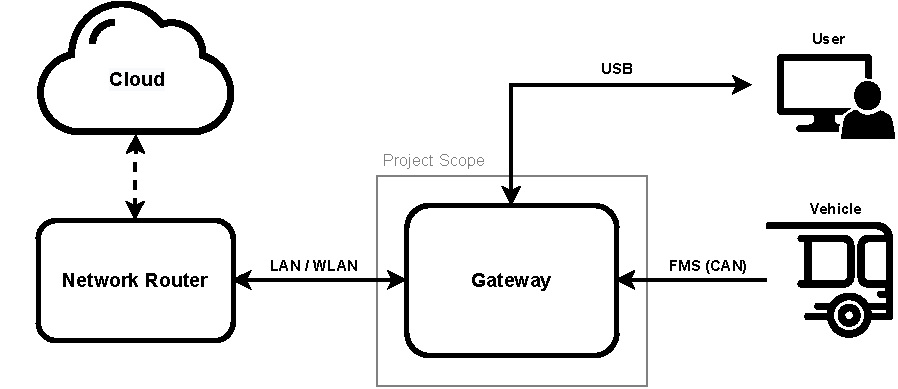
\includegraphics[height=5cm]{images/Block_Diagram}
	\caption{System Block Diagram}
	%\vspace{-2ex}
	%\caption*{\textbf{Source:} Original task definition}
	\label{fig:system_block_diagram}
\end{figure}

\acrshort{fms}-Packets are received and processed by the gateway. A configurable filter decides which packets get forwarded and limits the maximal transmission update rate. The network router acts as a receiver, which can upload the information  over the internet to a cloud-based system.
Device settings as well as the filter configuration can be updated by the user without the need of re-uploading a new firmware image. The user can access the device by an \acrshort{usb} interface. \newline
To gather additional motion data of the vehicle, an \acrfull{imu} will be integrated.
The collected motion data gets processed and will be available for further usage. \newline
\newline
Various use cases were defined in \cref{sec:use_cases}.